This section evaluates the performance of \textsc{Daf-Cl}, focusing on the F1 score.
Our evaluation covers the following aspects:
\begin{itemize}
	\item 
	\item 
	\item
\end{itemize}

\subsection{Datasets}  \label{subsec: data}

The proposed \textsc{Daf-Cl} framework addresses four-class speech emotion recognition, where each utterance is classified into one of four emotion categories: \textit{happy}, \textit{sad}, \textit{angry}, and \textit{neutral}. To improve the robustness and generalization capability of the proposed framework across different recording conditions, speakers, and speaking styles, a unified corpus was constructed by integrating several publicly available emotional speech datasets.

Speech utterances were collected from MELD \cite{MELD2019}, CREMA-D \cite{Cao2014}, IEMOCAP \cite{Busso2008}, Morgan Emotional Speech Set (MESS) \cite{MESS2019}, TESS \cite{Pichora_2020}, ASVP-ESD \cite{2020asvpesd}, and JL Corpus \cite{JL2018}. As summarized in Table~\ref{tab:dataset}, CREMA-D, MELD, and MESS provide both speech recordings and textual transcriptions, whereas the remaining datasets contain only speech audio. For datasets without textual annotations, transcriptions were automatically generated using the Whisper-large-v3 automatic speech recognition (ASR) model \cite{Radford2023}.

\begin{table}[ht]
	\centering
	\caption{Summary of the emotional speech datasets used to construct the proposed multimodal corpus.}
	\label{tab:dataset}
	
	\begin{tabular}{
			|>{\centering\arraybackslash}m{0.25\columnwidth}
			|>{\centering\arraybackslash}m{0.20\columnwidth}
			|>{\centering\arraybackslash}m{0.22\columnwidth}
			|>{\centering\arraybackslash}m{0.20\columnwidth}|
		}
		\hline
		\textbf{Dataset} &
		\textbf{Modality} &
		\textbf{Samples (Hours)} &
		\textbf{Speech Type} \\
		\hline
		\hline
		MELD & Audio + Text & 8,200 (7.2 h) & Conversational \\
		\hline
		CREMA-D & Audio + Text & 4,900 (3.5 h) & Read Speech \\
		\hline
		IEMOCAP & Audio & 4,490 (5.6 h) & Conversational \\
		\hline
		MESS & Audio + Text & 1,800 (1.45 h) & Read Speech \\
		\hline
		TESS & Audio & 1,600 (1.0 h) & Read Speech \\
		\hline
		ASVP-ESD & Audio & 1,000 (0.8 h) & Conversational \\
		\hline
		JL Corpus & Audio & 800 (0.5 h) & Read Speech \\
		\hline
	\end{tabular}
\end{table}

The resulting corpus comprises approximately 22,790 utterances (around 20 hours of speech) and includes both acted and spontaneous conversational speech. Specifically, CREMA-D, TESS, JL Corpus and MESS primarily capture prosodic variations under controlled recording conditions, whereas IEMOCAP, MELD, and ASVP-ESD contain more natural conversational interactions, thereby providing greater diversity in emotional expression.

Since the MELD recordings frequently contain high-energy laughter segments that may interfere with speech emotion recognition, the Whisper Speech Event Detection (Whisper-SED) model \cite{Yuan2023} was employed to automatically detect and remove laughter regions prior to feature extraction.

The corpus was partitioned into training, validation, and testing subsets while enforcing speaker independence between the training and testing sets. In addition, emotion-stratified sampling was adopted to preserve the class distribution across all partitions. Specifically, 10\% of the corpus was reserved as an independent test set, while the remaining 90\% was used for five-fold cross-validation. A separate \textsc{Daf-Cl} model was trained on each fold, resulting in an ensemble of five models. During inference, the final prediction was obtained by averaging the output logits of the five models, thereby reducing prediction variance and improving robustness.

\subsection{Experimental Setup and Implementation Details}

The proposed \textsc{Daf-Cl} framework is implemented using PyTorch and the PyTorch Lightning framework. Following the data partition described in Section \ref{subsec: data}, the training set is partitioned into five folds, where five independent \textsc{Daf-Cl} models are trained for 10 epochs using a five-fold cross-validation protocol. During inference, the prediction logits produced by the five models are averaged to obtain the final emotion prediction for each test utterance. This ensemble strategy improves prediction stability and reduces the variance associated with a single trained model.

 All speech audio signals are uniformly resampled to 16,000~Hz. To ensure a consistent computational cost and prevent excessively long recordings from dominating memory consumption, audio signals are truncated to a maximum duration of 10 seconds. Acoustic chunking is conducted via a sliding window configuration with a chunk size of $T_{\text{chunk}} = 3.0$~seconds and a hop overlap of 75\% ($0.75$). Any extracted chunk falling below the specified window length is zero-padded to maintain dimension uniformity. Textual transcripts are processed using the pre-trained RoBERTa tokenizer \cite{liu2019roberta}, where the maximum token length is restricted to 64 tokens per sequence.

The multi-layer acoustic backbone is initialized using the pre-trained \texttt{WavLM\_base\_plus} \cite{chen2022wavlm} checkpoint, while the textual branch leverages a pre-trained emotion-focused RoBERTa model \cite{liu2019roberta}. To preserve fundamental low-level acoustic representations while encouraging high-level task adaptation, the first four transformer encoder layers of the WavLM backbone are kept frozen throughout training ($\text{layer\_num} < 4$), leaving subsequent layers fully trainable. The layer-aggregation weights $\omega_l$ are initialized uniformly across all encoder layers. The temporal aggregation network utilizes a 2-layer vanilla Transformer Encoder configuration with a hidden dimension $D = 768$, 8 attention heads, a feed-forward network dimension of 2048, and a dropout rate of $0.2$. Both the acoustic and textual feature projection layers map their respective utterance embeddings into a shared contrastive latent space of dimension $D_{\text{proj}} = 256$.

End-to-end model optimization is conducted on two NVIDIA A100 GPUs, utilizing the AdamW optimizer \cite{Loshchilov2017} with a weight decay parameter of $0.005$ and a batch size of 4. To accommodate the disparate convergence properties of the deep pre-trained encoders and the custom structural decoder heads, different learning rates are assigned to the three network components to account for their different optimization dynamics: $\eta_{\text{enc}} = 2 \times 10^{-5}$ for acoustic encoder, $\eta_{\text{text}} = 5 \times 10^{-5}$ for textual encoder, and $\eta_{\text{dec}} = 1 \times 10^{-4}$ for fusion modules and projectors. 

The multi-task optimization objective is regularized by fixing the alignment loss weight to $\lambda_{\text{align}} = 0.15$ and the structured supervised contrastive learning loss weight to $\lambda_{\text{supcon}} = 0.15$. The supervised contrastive loss employs a temperature parameter of $\tau = 0.05$. Class imbalance is addressed using class-balanced weights computed from the training partition and incorporated into the cross-entropy classification loss ($\mathcal{L}_{\text{ce}}$). For each fold, the checkpoint achieving the highest validation Macro $F_1$ is retained. The five retained models are subsequently combined during inference using logit averaging.

\subsection{Results and Discussion}
\subsubsection{Performance on the Test Set}
After training, the \textsc{Daf-Cl} model was evaluated on the test set described in Section~\ref{subsec: data}. The model achieved a macro-averaged F1 score of 87.37\%. As shown in Figure~\ref{fig:cm}, the model correctly classified most test instances, although some misclassification was observed, particularly between the \textit{happy} and \textit{neutral} classes. The classification report presented in Table~\ref{tab:report} further indicates that the \textit{angry} and \textit{sad} classes achieved the highest F1 scores, whereas the \textit{neutral} and \textit{happy} classes obtained comparatively lower scores. These findings suggest that the model performs consistently across most emotion classes; however, distinguishing between acoustically and semantically similar emotions remains challenging because emotional expressions may overlap in certain contexts.

\begin{figure}
	\centering
	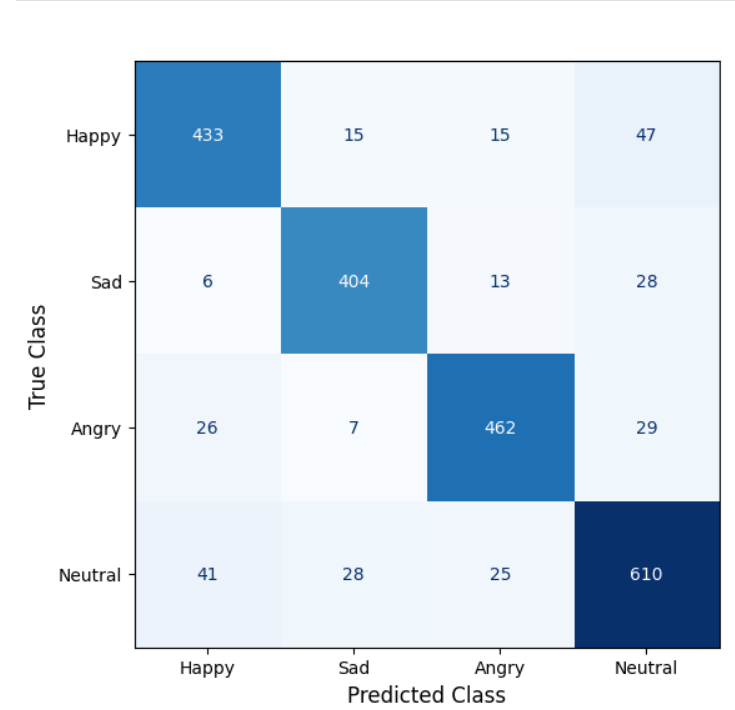
\includegraphics[width=1\linewidth]{cm}
	\caption{Confusion matrix of the \textsc{Daf-Cl} model.}
	\label{fig:cm}
\end{figure}

\begin{table}[ht]
	\centering
	\caption{\textsc{Daf-Cl} classification report.}
	\label{tab:report}
	
	\begin{tabular}{
			|>{\centering\arraybackslash}m{0.25\columnwidth}
			|>{\centering\arraybackslash}m{0.20\columnwidth}
			|>{\centering\arraybackslash}m{0.20\columnwidth}
			|>{\centering\arraybackslash}m{0.20\columnwidth}|
		}
		\hline
		\textbf{Classes} &
		\textbf{Precision \%} &
		\textbf{Recall \%} &
		\textbf{F1 Score \%} \\
		\hline
		\hline
		Happy & 85.43 & 86.65 & 86.04 \\
		\hline
		Sad & 89.71 & 88.71 & 88.93 \\
		\hline
		Angry & 88.99 & 89.58 & 89.28 \\
		\hline
		Neutral & 85.57 & 84.90 & 85.24 \\
		\hline
	\end{tabular}
\end{table}

\subsubsection{Comparison with Related Work}

To highlight the effectiveness of the proposed \textsc{Daf-Cl} framework, its performance was compared with recent multimodal emotion recognition methods that incorporate various contrastive learning strategies \cite{qian2022, Kim2023, Shi2024, Nguyen2024}, as reviewed in Section~\ref{sec:related work}. These studies were selected because they evaluate the same emotion classes considered by \textsc{Daf-Cl} and report results on the widely used IEMOCAP~\cite{Busso2008} and MELD~\cite{MELD2019} datasets. Tables~\ref{tab:Iemocap} and~\ref{tab:Meld} present the comparative results on the IEMOCAP and MELD datasets, respectively. Since the evaluation metrics reported by previous studies differ, the comparison is presented using the metrics available in the corresponding publications to ensure a fair and transparent evaluation.


\begin{table*}[ht]
	\centering
	\caption{Comparison of \textsc{Daf-Cl} with recent multimodal emotion recognition methods on the IEMOCAP dataset.}
	\label{tab:Iemocap}
	
	\begin{tabular}{
			|>{\centering\arraybackslash}m{0.8\columnwidth}
			|>{\centering\arraybackslash}m{0.2\columnwidth}
			|>{\centering\arraybackslash}m{0.2\columnwidth}
			|>{\centering\arraybackslash}m{0.2\columnwidth}|
		}
		\hline
		\textbf{Method} &
		\textbf{Weighted Accuracy (\%)} &
		\textbf{Unweighted Accuracy (\%)} &
		\textbf{Weighted F1 (\%)} \\
		\hline
		\hline
		Contrastive regularization for multimodal emotion recognition using audio and text \cite{qian2022} &
		76.06 &
		77.45 &
		-- \\
		\hline
		
		Enhancing emotion recognition in conversation through emotional coss-modal fusion and inter-class contrastive learning \cite{Shi2024} &
		68.77 &
		-- &
		68.66 \\
		\hline
		
		Focus-attention-enhanced crossmodal transformer with metric learning for multimodal speech emotion recognition \cite{Kim2023} &
		77.4 &
		77.7 &
		-- \\
		\hline
		
		
		HuBERT-CLAP: contrastive learning-based multimodal emotion recognition using self-alignment approach \cite{Nguyen2024} &
		77.22 &
		-- &
		-- \\
		\hline
		
		\textsc{\textbf{Daf-Cl} (Proposed)}: a robust multimodal emotion classification framework with dynamic adaptive fusion and contrastive learning &
		81.50 &
		82.92 &
		81.88 \\
		\hline
		
		\hline
	\end{tabular}
\end{table*}

\begin{table*}[ht]
	\centering
	\caption{Comparison of \textsc{Daf-Cl} with recent multimodal emotion recognition methods on the MELD dataset.}
	\label{tab:Meld}
	
	\begin{tabular}{
			|>{\centering\arraybackslash}m{0.8\columnwidth}
			|>{\centering\arraybackslash}m{0.2\columnwidth}
			|>{\centering\arraybackslash}m{0.2\columnwidth}
			|>{\centering\arraybackslash}m{0.2\columnwidth}|
		}
		\hline
		\textbf{Method} &
		\textbf{Accuracy (\%)} &
		\textbf{Weighted F1 (\%)} \\
		\hline
	
		Enhancing emotion recognition in conversation through emotional coss-modal fusion and inter-class contrastive learning \cite{Shi2024} &
		65.62 &
		64.73\\
		\hline
		
		\textsc{\textbf{Daf-Cl} (Proposed)}: a robust multimodal emotion classification framework with dynamic adaptive fusion and contrastive learning &
		81.66 &
		81.55 \\
		\hline
		
		\hline
	\end{tabular}
\end{table*}

As shown in Tables~\ref{tab:Iemocap} and~\ref{tab:Meld}, the proposed \textsc{Daf-Cl} framework consistently outperforms recent multimodal emotion recognition methods based on contrastive learning. On the IEMOCAP dataset, \textsc{Daf-Cl} achieves the highest performance across the reported evaluation metrics. Compared with the highest previously reported weighted accuracy of 77.40\%~\cite{Kim2023}, \textsc{Daf-Cl} improves the weighted accuracy by 4.10 percentage points. Similarly, the proposed framework improves the highest reported unweighted accuracy by 5.22 percentage points. These improvements demonstrate the effectiveness of combining dynamic adaptive fusion with contrastive learning to learn more discriminative multimodal representations.

A similar trend is observed on the MELD dataset, where \textsc{Daf-Cl} outperforms the most recent contrastive learning-based method by approximately 16 percentage points. The consistent improvements on both the acted IEMOCAP dataset and the conversational MELD dataset indicate that the proposed framework effectively exploits the complementary information provided by the acoustic and textual modalities, resulting in robust and generalizable multimodal emotion representations.
 

\subsubsection{Generalization to Unseen Datasets}
To further evaluate the robustness and generalization capability of \textsc{Daf-Cl}, the proposed model was evaluated on three completely unseen datasets: Emotional-EMA~\cite{ema}, EmoV-DB-sorted~\cite{emov}, and Emo-DB~\cite{emodb}. None of these datasets was used during training, and they contain different speakers and data distributions. Table~\ref{tab:unseen_results} summarizes the evaluated emotion classes, the number of recordings, and the corresponding F1 scores obtained by \textsc{Daf-Cl}. The results demonstrate that the proposed framework maintains consistently high performance across unseen datasets, indicating good generalization to previously unseen speakers and recording conditions.

Furthermore, the model achieved an F1 score of 90\% on the German Emo-DB dataset despite being trained primarily on English emotional speech corpora. This result suggests that the proposed framework exhibits a degree of cross-lingual generalization, although a more comprehensive evaluation on additional languages is required to fully assess its multilingual robustness.


\begin{table}[ht]
	\centering
	\caption{Generalization performance of \textsc{Daf-Cl} on unseen emotion recognition datasets.}
	\label{tab:unseen_results}
	
	\begin{tabular}{
			|>{\centering\arraybackslash}m{0.24\columnwidth}
			|>{\centering\arraybackslash}m{0.28\columnwidth}
			|>{\centering\arraybackslash}m{0.19\columnwidth}
			|>{\centering\arraybackslash}m{0.16\columnwidth}|
		}
		\hline
		\textbf{Dataset} &
		\textbf{Emotion Classes} &
		\textbf{Number of Recordings} &
		\textbf{F1 Score (\%)} \\
		\hline
		\hline
		Emotional-EMA &
		Happy, Sad, Angry, Neutral &
		680 &
		87 \\
		\hline
		
		EmoV-DB-sorted &
		Angry, Neutral &
		2,836 &
		93 \\
		\hline
		
		Emo-DB &
		Happy, Sad, Angry, Neutral &
		339 &
		90 \\
		\hline
	\end{tabular}
\end{table}



\subsection{Ablation Study}

To evaluate the contribution of each component in the proposed \textsc{Daf-Cl} framework, an ablation study was conducted by progressively extending a baseline model with the proposed modules while keeping all training settings unchanged. All experiments were performed on the same test set described in Section~\ref{subsec: data}, and performance was evaluated using the F1 score. This analysis quantifies the individual contribution of each module and demonstrates how the proposed components collectively improve the overall classification performance.

In addition to the progressive ablation study, several architectural design choices were investigated to justify the proposed implementation. Specifically, alternative variants of the chunk aggregation strategy, fusion strategy, layer adaptive weighting mechanism, and emotion similarity matrix were evaluated while keeping the remaining components unchanged. The results provide further insight into the impact of each design choice on the overall performance of \textsc{Daf-Cl}.

\subsubsection{Progressive Ablation Study}

The contribution of each component in the proposed \textsc{Daf-Cl} framework was evaluated through a progressive ablation study. Starting from a simplified multimodal baseline, one component was added at a time until the full proposed architecture was obtained. The baseline model uses the final hidden layer of WavLM instead of adaptive layer fusion, aggregates chunk-level audio representations using mean pooling, and combines the audio and text modalities through late fusion with a fixed weight of 0.5 for each modality. Both the cross-modal alignment loss and the structured supervised contrastive learning (SSCL) objective are excluded from the baseline.

Starting from this baseline, the following components were incrementally incorporated: (1) \textit{adaptive layer fusion}, which replaces the final WavLM hidden state with a learned weighted combination of multiple hidden layers; (2) \textit{chunk weighting}, which replaces uniform mean pooling with a learnable chunk aggregation strategy based on the gate $\alpha$ and classifier confidence; (3) \textit{dynamic fusion}, which replaces fixed modality weighting with an input-dependent fusion coefficient; (4) \textit{cross-modal alignment}, which introduces an alignment loss between utterance-level audio and text embeddings; and (5) \textit{SSCL}, which adds the proposed structured supervised contrastive learning objective using an emotion similarity matrix over audio chunk representations.

As shown in Table~\ref{tab:ablation}, adaptive layer fusion provides a clear improvement over the baseline, increasing the macro F1 score from 78.4\% to 82.3\%. This indicates that aggregating information from multiple WavLM layers is more effective than relying only on the final hidden layer. After adding chunk weighting, the macro F1 score slightly decreases to 81.4\%. This suggests that chunk-level weighting alone may not be sufficient when the audio embedding space is not yet well structured. However, when dynamic fusion is introduced, the performance increases to 82.9\%, indicating that input-dependent modality weighting helps the model adjust the contribution of audio and text according to the reliability of each utterance.

Adding cross-modal alignment further improves the macro F1 score to 84.8\%, demonstrating the benefit of reducing the representation gap between the audio and textual embedding spaces. Finally, incorporating SSCL leads to the best overall performance, achieving a macro F1 score of 87.4\%. This result shows that explicitly modeling structured relationships among emotion classes strengthens the discriminative quality of the learned audio representations. Overall, the full \textsc{Daf-Cl} framework improves the macro F1 score by 9.0 percentage points over the baseline, confirming that the proposed components are complementary and jointly contribute to the final performance.

\begin{table*}[ht]
	\centering
	\caption{Progressive ablation study of the proposed \textsc{Daf-Cl} framework. Each model variant incrementally incorporates one additional component while keeping all other training settings unchanged.}
	\label{tab:ablation}
	\begin{tabular}{
			|l|
			>{\centering\arraybackslash}m{0.16\columnwidth}|
			>{\centering\arraybackslash}m{0.16\columnwidth}|
			>{\centering\arraybackslash}m{0.16\columnwidth}|
			>{\centering\arraybackslash}m{0.18\columnwidth}|
			>{\centering\arraybackslash}m{0.18\columnwidth}|
			>{\centering\arraybackslash}m{0.14\columnwidth}|
		}
		\hline
		\textbf{Model Variant} &
		\textbf{Adaptive Layer Fusion} &
		\textbf{Chunk Weighting} &
		\textbf{Dynamic Fusion} &
		\textbf{Cross-modal Alignment} &
		\textbf{SSCL} &
		\textbf{Macro F1 (\%)} \\
		\hline
		Baseline &
		-- & -- & -- & -- & -- &
		78.4 \\
		\hline
		+ Adaptive Layer Fusion &
		$\checkmark$ & -- & -- & -- & -- &
		82.3 \\
		\hline
		+ Chunk Weighting &
		$\checkmark$ & $\checkmark$ & -- & -- & -- &
		81.4 \\
		\hline
		+ Dynamic Fusion &
		$\checkmark$ & $\checkmark$ & $\checkmark$ & -- & -- &
		82.9 \\
		\hline
		+ Cross-modal Alignment &
		$\checkmark$ & $\checkmark$ & $\checkmark$ & $\checkmark$ & -- &
		84.8 \\
		\hline
		+ SSCL (Proposed) &
		$\checkmark$ & $\checkmark$ & $\checkmark$ & $\checkmark$ & $\checkmark$ &
		\textbf{87.4} \\
		\hline
	\end{tabular}
\end{table*}


\subsubsection{Impact of the Chunk Aggregation Strategy} \label{subsec: chunk}
To justify our chunk aggregation design choice, we evaluate five alternative strategies for combining chunk-level predictions into an utterance-level representation, under an otherwise identical training configuration. For the mean pooling, max pooling, and confidence-only variants, audio and text logits are combined using a fixed, equally weighted fusion (0.5 for each modality), since these variants do not produce a learned per-utterance gate for dynamic fusion. Table~\ref{tab:chunkimpact} reports the resulting macro F1 scores.

As shown, simple pooling strategies (mean and max) yield the weakest performance, since they treat all chunks as equally informative regardless of their acoustic content or the classifier's certainty about them. The learned gate ($\alpha$ only) improves modestly over pooling, but its capacity is limited: $\alpha$ is learned solely from the chunk's acoustic embedding and has no access to how the classifier is currently behaving on that chunk, making it prone to relying on superficial acoustic cues rather than a reliable indicator of chunk informativeness. Confidence-only weighting performs better still, as it is derived directly from the classifier's own output entropy and therefore adapts to the model's evolving decision boundary; however, it cannot by itself distinguish genuinely informative chunks from chunks on which the classifier is confidently wrong. Combining the two signals ($\text{confidence} \times \alpha$) consistently yields the best performance, as the two mechanisms compensate for each other's weaknesses: a chunk receives high weight only when it is both acoustically salient (high $\alpha$) and one on which the classifier currently expresses low uncertainty (high confidence), effectively penalizing chunks that would otherwise mislead the final prediction. This joint criterion proves more robust than either signal in isolation.

\begin{table}[ht]
	\centering
	\caption{Impact of chunk aggregation strategy on macro F1 score.}
	\label{tab:chunkimpact}
	\begin{tabular}{
			|l|
			>{\centering\arraybackslash}m{0.30\columnwidth}|
		}
		\hline
		\textbf{Chunk Aggregation Method} &
		\textbf{Macro F1 (\%)} \\
		\hline
		Mean pooling &
		83.1  \\
		\hline
		Max pooling &
		82.9 \\
		\hline
		Learned $\alpha$ only &
		83.4 \\
		\hline
		Confidence only &
		84.1 \\
		\hline
		Confidence $\times$ $\alpha$ (proposed) &
		\textbf{87.4} \\
		\hline
	\end{tabular}
\end{table}

\subsubsection{Impact of the Fusion Strategy}

To evaluate the effectiveness of the proposed fusion strategy, four multimodal fusion approaches were compared: (1) \textit{early fusion}, where the audio and text embeddings are concatenated at the feature level and processed by a shared classification head; (2) \textit{late fusion with equal weighting}, where each modality is classified independently and the predicted logits are combined using a fixed weight of 0.5 for each modality; (3) \textit{late fusion with a dedicated learnable gate}, where a separate gating network jointly processes the audio and text embeddings to estimate the fusion weight; and (4) the proposed \textit{dynamic fusion} strategy in \textsc{Daf-Cl}, which also performs late fusion with a learnable gate but reuses the weighting coefficient, $\alpha$, learned during chunk aggregation instead of introducing an additional cross-modal gating network. Unlike the dedicated learnable gate, which must learn the relative importance of the two modalities from scratch, the proposed approach reuses the weighting coefficient learned during chunk aggregation, which provides a reliability-aware signal for the acoustic representation.

Table \ref{tab:fusionimpact} presents the macro F1 scores obtained using each fusion strategy. Early fusion achieves the lowest performance in this experimental setting, suggesting that directly concatenating the audio and textual representations may not be sufficient to fully exploit their complementary information within the proposed framework. Late fusion with equal weighting improves the classification performance in this setting, suggesting that allowing each modality to make an independent prediction before combining their outputs is more effective than direct feature-level concatenation for the evaluated task. This suggests that learning an additional cross-modal gating function may increase the optimization difficulty and reduce generalization under the available training data. In contrast, the proposed dynamic fusion strategy achieves the highest macro F1 score. By reusing the chunk-level weighting coefficient as the fusion weight, the proposed framework avoids introducing an additional gating network while exploiting a reliability-aware signal learned during chunk aggregation. This leads to a more stable and effective multimodal fusion mechanism, as reflected by the highest macro F1 score in Table~\ref{tab:fusionimpact}.

\begin{table}[ht]
	\centering
	\caption{Impact of different fusion strategies on macro F1 score.}
	\label{tab:fusionimpact}
	\begin{tabular}{
			|l|
			>{\centering\arraybackslash}m{0.30\columnwidth}|
		}
		\hline
		\textbf{Fusion Strategy} &
		\textbf{Macro F1 (\%)} \\
		\hline
		Early fusion &
		83.7 \\
		\hline
		Late fusion with equal weighting &
		85.7 \\
		\hline
		Late fusion with dedicated learnable gate &
		85.0 \\
		\hline
		Proposed dynamic fusion &
		\textbf{87.4} \\
		\hline
	\end{tabular}
\end{table}

\subsubsection{Impact of the Layer Aggregation Strategy}

To justify our choice of layer aggregation strategy, we compare three variants for combining the $L$ hidden layers produced by the audio encoder: (1) using only the \textit{last hidden layer}, a common choice in prior speech emotion recognition literature; (2) \textit{averaging all hidden layers} uniformly; and (3) our proposed \textsc{Daf-Cl} \textit{adaptive layer weighting}, which learns a softmax-normalized weight for each layer and combines them via a weighted sum, allowing the model to determine the contribution of each layer directly from the training data.

Table~\ref{tab:layerimpact} reports the macro F1 score for each variant. Under our training setting, incorporating information from all layers substantially outperforms relying on the last layer alone, indicating that emotion-relevant information is distributed across the encoder's depth rather than concentrated solely in its final representation. The proposed adaptive weighting further improves over uniform averaging, showing that allowing the model to learn a layer-specific weighting, rather than treating all layers as equally informative, provides a consistent advantage.

\begin{table}[ht]
	\centering
	\caption{Impact of layer aggregation strategy on macro F1 score.}
	\label{tab:layerimpact}
	\begin{tabular}{
			|l|
			>{\centering\arraybackslash}m{0.30\columnwidth}|
		}
		\hline
		\textbf{Layer Representation} &
		\textbf{Macro F1 (\%)} \\
		\hline
		Last hidden layer &
		82.30  \\
		\hline
		Average all layers &
		86.50 \\
		\hline
		Proposed adaptive weighting &
		87.40 \\
		\hline
	\end{tabular}
\end{table}

To better understand what the adaptive weighting mechanism learns, we inspect the softmax-normalized layer weights $\text{softmax}(\mathbf{w})$ from the trained model, shown in Figure~\ref{fig:layerweights}. The learned weights assign a mild but consistent preference to the upper-middle layers of the encoder, peaking at layer 10 (weight $= 0.103$), while the earliest layers (1--7) and the final layer (12) receive weights slightly below the uniform baseline ($1/L = 0.083$). Notably, no single layer dominates the aggregation: all weights remain within a narrow range (0.074--0.103), indicating that the model retains and combines information from nearly all layers rather than collapsing onto a small subset. This suggests that the performance gain from adaptive weighting stems from a mild, learned redistribution of emphasis across layers rather than from discarding most of the encoder's depth, which is consistent with the observation that averaging all layers already performs close to the proposed method (Table~\ref{tab:layerimpact}). The relatively lower weight assigned to the final layer is consistent with prior findings that the last layers of self-supervised speech encoders tend to specialize toward the pretraining objective rather than downstream paralinguistic tasks \cite{pepino21_interspeech}, making upper-middle layers a more informative source for emotion-discriminative features in this setting.

\begin{figure}[ht]
	\centering
	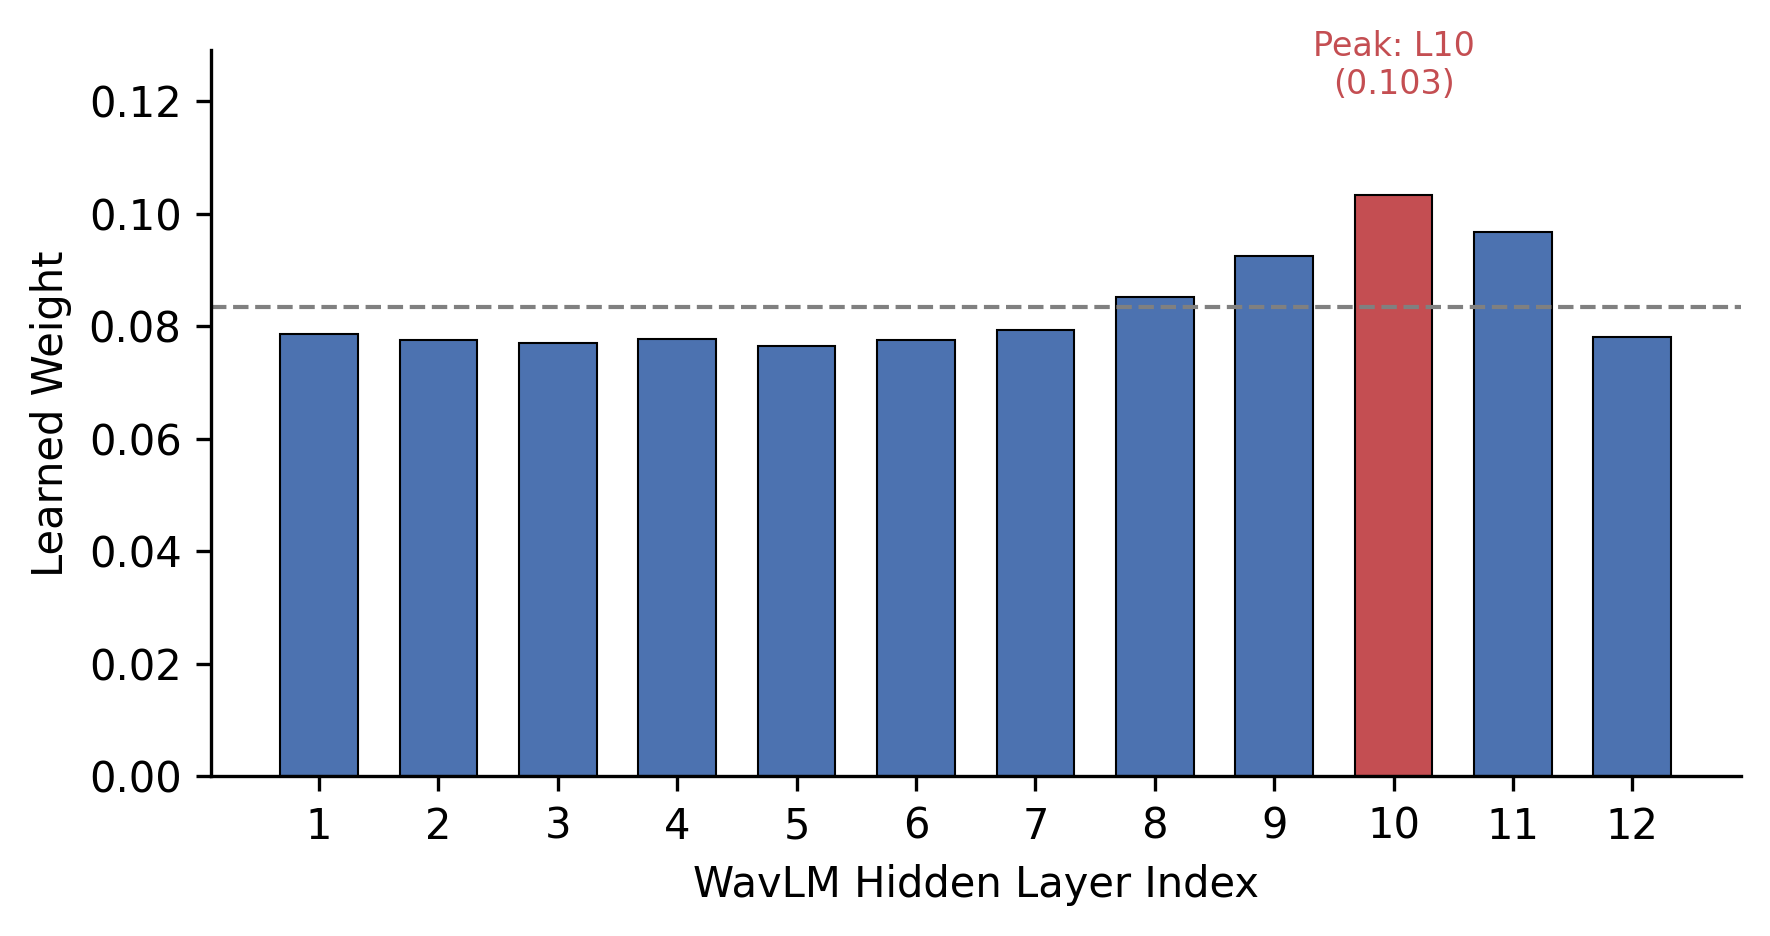
\includegraphics[width=0.85\columnwidth]{layer_weights.png}
	\caption{Learned adaptive layer weights (softmax-normalized) across the 12 WavLM hidden layers. The dashed line marks the uniform weight ($1/L$) for reference; layers above it contribute more to the fused representation than a simple average would assign, while layers below it contribute less.}
	\label{fig:layerweights}
\end{figure}

\subsubsection{Impact of the Emotion Similarity Matrix} 

To evaluate the contribution of the proposed emotion similarity matrix, we compare the structure supervised contrastive loss (SSCL) with the standard supervised contrastive loss (SupCon)~\cite{khosla2020supervised}. In standard SupCon, samples from the same class are treated as positive pairs, whereas samples from different classes are treated as negative pairs. This hard positive/negative formulation ignores the graded relationships that may exist between emotion classes. In contrast, the proposed formulation incorporates an emotion similarity matrix into the contrastive objective to model soft inter-class relationships.

It should be emphasized that the proposed similarity matrix is used only within the contrastive learning objective to regularize the learned audio embedding space; it does not modify the ground-truth labels or the final classification objective. Thus, the classifier is still optimized to distinguish the target emotion categories, while the contrastive objective encourages the audio representation to preserve meaningful similarities among emotionally related classes. This is particularly relevant for speech emotion recognition, where emotions may overlap acoustically and perceptually rather than forming completely independent clusters.

As shown in Table~\ref{tab:emotionimpact}, incorporating the proposed emotion similarity matrix improves the macro F1 score compared with standard SupCon. This result suggests that preserving soft relationships among emotion classes provides a more informative supervision signal than treating all different-class pairs as equally dissimilar. By encoding these graded relationships, the proposed contrastive objective learns a more structured audio embedding space, which contributes to improved classification performance.

\begin{table}[ht]
	\centering
	\caption{Impact of the proposed emotion similarity matrix on macro F1 score.}
	\label{tab:emotionimpact}
	\begin{tabular}{
			|l|
			>{\centering\arraybackslash}m{0.30\columnwidth}|
		}
		\hline
		\textbf{SupCon Variant} &
		\textbf{Macro F1 (\%)} \\
		\hline
		Standard SupCon &
		86.20 \\
		\hline
		Proposed emotion similarity matrix &
		\textbf{87.40} \\
		\hline
	\end{tabular}
\end{table}


\subsection{Sensitivity Analysis}

To examine the robustness of \textsc{Daf-Cl} with respect to its main hyperparameters, a sensitivity analysis was conducted on the parameters that directly affect the proposed components. Specifically, we investigated the loss weighting coefficients $\lambda_{\text{align}}$ and $\lambda_{\text{SSCL}}$, which control the contribution of the cross-modal alignment loss and the structured supervised contrastive learning objective, respectively. In addition, the temperature parameter $\tau$ and the audio segmentation parameters, including chunk size and chunk overlap, were evaluated. Unless otherwise stated, all experiments were conducted under the same training and evaluation settings, and performance was measured using macro F1 score.

\subsubsection{Sensitivity to $\lambda_{\text{align}}$}

The coefficient $\lambda_{\text{align}}$ controls the contribution of the cross-modal alignment loss during training. This loss encourages the audio and textual representations of the same utterance to be closer in the shared embedding space. However, an excessively small value may limit the effect of alignment, whereas an overly large value may dominate the main classification objective. Therefore, different values of $\lambda_{\text{align}}$ were evaluated to identify a suitable balance between classification learning and cross-modal representation alignment.

As shown in Table \ref{tab:lambda_align}, the best macro F1 score is achieved when $\lambda_{\text{align}}=0.4$, which corresponds to the setting used in the proposed \textsc{Daf-Cl} framework. A smaller value, such as $\lambda_{\text{align}}=0.1$, results in lower performance, suggesting that weak alignment is insufficient to effectively reduce the gap between the audio and textual embedding spaces. Increasing the coefficient to 0.2 improves the performance, confirming the benefit of incorporating the alignment loss. However, further increasing the value to 0.6 slightly reduces the macro F1 score, indicating that assigning excessive weight to the alignment objective may negatively affect the discriminative learning required for emotion classification. These results suggest that $\lambda_{\text{align}}=0.4$ provides an effective trade-off between cross-modal alignment and classification performance.

\begin{table}[ht]
	\centering
	\caption{Sensitivity analysis of the cross-modal alignment loss coefficient $\lambda_{\text{align}}$.}
	\label{tab:lambda_align}
	\begin{tabular}{
			|>{\centering\arraybackslash}m{0.35\columnwidth}|
			>{\centering\arraybackslash}m{0.35\columnwidth}|
		}
		\hline
		\textbf{$\lambda_{\text{align}}$} &
		\textbf{Macro F1 (\%)} \\
		\hline
		0.1 & 84.42 \\
		\hline
		0.2 & 85.3 \\
		\hline
		0.4 & \textbf{87.40} \\
		\hline
		0.6 & 86.1 \\
		\hline
	\end{tabular}
\end{table}



\subsubsection{Sensitivity to $\lambda_{\text{SSCL}}$}

The coefficient $\lambda_{\text{SSCL}}$ controls the contribution of the structured supervised contrastive learning objective during training. This objective regularizes the learned audio representation by encouraging better separation between emotion classes while preserving the structured relationships defined by the emotion similarity matrix. However, assigning an insufficient weight may limit the effect of contrastive learning, whereas an excessively large value may overemphasize the auxiliary representation-learning objective at the expense of the main classification objective. Therefore, different values of $\lambda_{\text{SSCL}}$ were evaluated to identify an appropriate balance.

As shown in Table \ref{tab:lambda_sscl}, the best macro F1 score is obtained when $\lambda_{\text{SSCL}}=0.3$, which is the value adopted in the proposed \textsc{Daf-Cl} framework. A lower value, such as $\lambda_{\text{SSCL}}=0.1$, results in comparatively lower performance, suggesting that weak contrastive supervision may be insufficient to learn highly discriminative emotion representations. Increasing the coefficient to 0.2 improves the macro F1 score, confirming the benefit of the SSCL objective. However, further increasing the value to 0.5 slightly decreases performance, indicating that excessive emphasis on the auxiliary contrastive objective may reduce the model's ability to optimize the final classification task. Although $\lambda_{\text{SSCL}}=0.3$ yields the highest macro F1 score, the performance remains relatively stable across the evaluated range. This indicates that the SSCL objective consistently contributes to representation learning, while the selected value provides the best balance between enhancing emotion-class separability and preserving the optimization of the main classification objective.

\begin{table}[ht]
	\centering
	\caption{Sensitivity analysis of the structured supervised contrastive learning coefficient $\lambda_{\text{SSCL}}$.}
	\label{tab:lambda_sscl}
	\begin{tabular}{
			|>{\centering\arraybackslash}m{0.35\columnwidth}|
			>{\centering\arraybackslash}m{0.35\columnwidth}|
		}
		\hline
		\textbf{$\lambda_{\text{SSCL}}$} &
		\textbf{Macro F1 (\%)} \\
		\hline
		0.1 & 85.81 \\
		\hline
		0.2 & 86.15 \\
		\hline
		0.3 & \textbf{87.40} \\
		\hline
		0.5 & 86.65 \\
		\hline
	\end{tabular}
\end{table}


\subsubsection{Sensitivity to the Temperature Parameter $\tau$}

The temperature parameter $\tau$ controls the sharpness of the similarity distribution in the contrastive learning objective. A smaller value of $\tau$ increases the emphasis on hard positive and negative pairs, leading to stronger separation in the embedding space. In contrast, a larger value produces a smoother similarity distribution, which may reduce the discriminative effect of the contrastive objective. Following common settings in contrastive learning, values in the range of 0.05 to 0.2 were evaluated.

As shown in Table \ref{tab:tau_sensitivity}, the best macro F1 score is achieved when $\tau=0.07$, which is the value adopted in the proposed \textsc{Daf-Cl} framework. Reducing the temperature to 0.05 slightly decreases performance, suggesting that excessive sharpening of the similarity distribution may overemphasize difficult pairs. Increasing $\tau$ to 0.1 and 0.2 leads to a larger performance reduction, indicating that a smoother similarity distribution weakens the ability of the contrastive objective to learn sufficiently discriminative emotion representations. These results show that $\tau=0.07$ provides the most effective balance between hard-pair emphasis and stable representation learning.

\begin{table}[ht]
	\centering
	\caption{Sensitivity analysis of the temperature parameter $\tau$.}
	\label{tab:tau_sensitivity}
	\begin{tabular}{
			|>{\centering\arraybackslash}m{0.35\columnwidth}|
			>{\centering\arraybackslash}m{0.35\columnwidth}|
		}
		\hline
		\textbf{$\tau$} &
		\textbf{Macro F1 (\%)} \\
		\hline
		0.05 & 86.19 \\
		\hline
		0.07 & \textbf{87.40} \\
		\hline
		0.10 & 85.55 \\
		\hline
		0.20 & 85.00 \\
		\hline
	\end{tabular}
\end{table}


\subsubsection{Sensitivity to Chunk Size}

The proposed \textsc{Daf-Cl} framework segments each audio utterance into fixed-length chunks to capture local emotional cues while supporting the processing of longer recordings. The chunk representations are subsequently aggregated to obtain an utterance-level acoustic representation. Considering the duration distribution of the training data, where the average utterance length is approximately 3~s, three chunk sizes of 2, 3, and 4~s were evaluated to examine the trade-off between temporal resolution and contextual coverage.

As shown in Table~\ref{tab:chunk_sensitivity}, the performance remains relatively stable across the evaluated chunk sizes, indicating that \textsc{Daf-Cl} is not highly sensitive to moderate variations in this parameter. A chunk size of 3~s achieves the highest macro F1 score of 87.40\% and is therefore adopted in the proposed framework. Shorter 2~s chunks provide finer temporal resolution but may capture less contextual information, whereas longer 4~s chunks provide broader context at the cost of reduced temporal granularity. The results suggest that a 3~s chunk size provides an appropriate balance between local emotional information and utterance-level context for the evaluated data.

\begin{table}[ht]
	\centering
	\caption{Sensitivity analysis of the audio chunk size.}
	\label{tab:chunk_sensitivity}
	\begin{tabular}{
			|>{\centering\arraybackslash}m{0.35\columnwidth}|
			>{\centering\arraybackslash}m{0.35\columnwidth}|
		}
		\hline
		\textbf{Chunk Size (s)} &
		\textbf{Macro F1 (\%)} \\
		\hline
		2 & 86.27 \\
		\hline
		3 & \textbf{87.40} \\
		\hline
		4 & 86.68 \\
		\hline
	\end{tabular}
\end{table}



\subsubsection{Sensitivity to Chunk Overlap}

To reduce the risk of losing emotionally relevant information at chunk boundaries, adjacent audio segments were processed with temporal overlap. Increasing the overlap provides greater continuity between neighboring chunks and allows transitional acoustic cues to be captured by more than one segment. However, excessive overlap also increases redundancy and computational cost. Therefore, overlap ratios of 0.25, 0.50, and 0.75 were evaluated to examine the trade-off between classification performance and processing efficiency.

As shown in Table~\ref{tab:chunk_overlap}, the lowest overlap ratio of 0.25 results in a lower macro F1 score, suggesting that limited overlap may omit useful contextual information around chunk boundaries. Increasing the overlap to 0.50 substantially improves performance, while a further increase to 0.75 does not provide an additional benefit and yields a comparable macro F1 score. Based on this result, an overlap ratio of 0.50 is adopted in the proposed \textsc{Daf-Cl} framework, as it provides the best observed performance while avoiding the additional redundancy and computational overhead associated with a larger overlap.

\begin{table}[ht]
	\centering
	\caption{Sensitivity analysis of the audio chunk overlap ratio.}
	\label{tab:chunk_overlap}
	\begin{tabular}{
			|>{\centering\arraybackslash}m{0.35\columnwidth}|
			>{\centering\arraybackslash}m{0.35\columnwidth}|
		}
		\hline
		\textbf{Chunk Overlap} &
		\textbf{Macro F1 (\%)} \\
		\hline
		0.25 & 85.10 \\
		\hline
		0.50 & \textbf{87.40} \\
		\hline
		0.75 & 87.00 \\
		\hline
	\end{tabular}
\end{table}


\subsection{Representation Analysis}

To qualitatively investigate the effect of the proposed structured supervised contrastive learning (SSCL) objective on the learned audio representation space, t-SNE was applied to the chunk-level audio embeddings obtained before and after incorporating SSCL. A balanced subset of 1,000 embeddings was randomly selected from the evaluation set, comprising 250 samples from each emotion class. The same samples and t-SNE configuration were used for both models to enable a consistent visual comparison.

Figure~\ref{fig:tsne_sscl} illustrates the resulting two-dimensional embedding distributions. Without SSCL, substantial overlap can be observed among the emotion classes, indicating limited structure in the learned audio representation space. After incorporating SSCL, the embeddings exhibit more compact within-class distributions and more distinguishable inter-class organization. Nevertheless, some overlap remains, particularly between the \textit{happy} and \textit{neutral} classes. This pattern is consistent with the classification results, where these two classes exhibit greater confusion and comparatively lower class-level performance than the other emotion categories.

The observed change in the embedding distribution provides qualitative support for the role of SSCL in organizing the audio representation space. In particular, the structured contrastive objective encourages discriminative class representations while preserving graded relationships among emotionally similar classes through the proposed emotion similarity matrix. This observation is also consistent with the performance improvements reported in the ablation study. Since t-SNE is a nonlinear dimensionality-reduction technique and does not directly quantify class separability, the visualization is used as complementary qualitative evidence rather than as an independent measure of representation quality.

\begin{figure*}[ht]
	\centering
	\begin{tabular}{cc}
		\includegraphics[width=0.85\columnwidth]{"tsne_without_sscl (1)"} & 
		\includegraphics[width=0.85\columnwidth]{"tsne_with_sscl (1)"} \\
		\small{(a) Without SSCL} &
		\small{(b) With SSCL}
	\end{tabular}
	\caption{t-SNE visualization of the chunk-level audio embedding space without and with the proposed SSCL objective. The same balanced subset of 1,000 embeddings (250 per emotion class) is used in both visualizations.}
	\label{fig:tsne_sscl}
\end{figure*}

